\documentclass[mim_thesis.tex]{subfiles} 
\begin{document}

The subsections on this chapter explain how to create an account on ADL Designer, the web-tool used for parsing the openEHR resources and how to connect a repository with it. Are also explained the steps taken for the development of the script made for archetypes compliance and comparison from a local repository with the GitHub mirror of openEHR CKM.  


\section{Programming Technologies}
After analyzed all the materials that were provided, was decided that the best platform for the script would be by using an web browser because of its practicality. For that, it was used the Angular 2 framework, together with the REST API calls that could be made to ADL Designer web tool which works as a middleware for fetching resources from the local repositories and to GitHub openEHR CKM repository, along with all the materials mentioned on \textit{Materials and Methods} chapter. For this was created a web-page that can run this script in the background, after using the credentials from ADL Designer for login and authentication.


\subsection{Script process and methodology}

Before running the script, it is necessary to create an account on ADL Designer and connect the local repository to it. If the repository of openEHR resources is not connected to this tool, the script it will not work, since it is dependent from it.

\subsubsection{Creating an account}
The official web-page for ADL Designer is \url{https://ehrscape.marand.si/designerv2}. It has a default account that can be logged in for testing purposes. To have a personal account is necessary to request it at \url{https://www.ehrscape.com/register.html}.
After getting an account, it is necessary to connect the desired repository to ADL Designer. It offers connection to various cloud repositories like OneDrive, Google Drive, Dropbox, GitHub, Bitbucket, Box and other CVS systems like GIT or connection to a local folder in a local machine. Depending on the chosen repository, other fields needs to be filled up as seen in figure \ref{fig:adl_designer_repositories}

\begin{figure}[H]
	\centering
    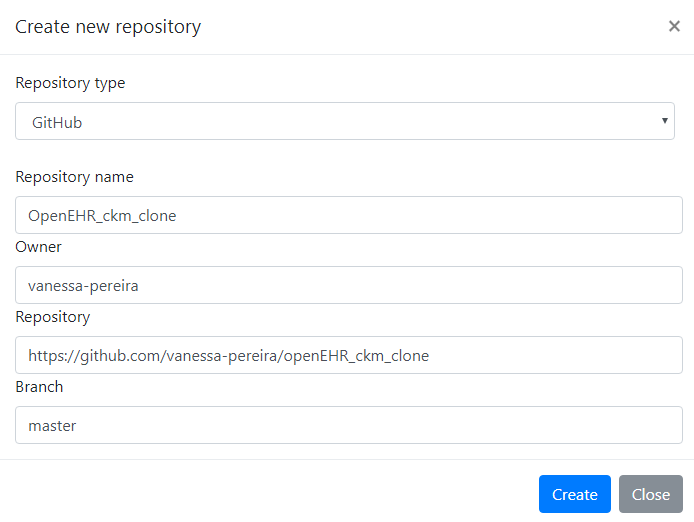
\includegraphics[width=1\textwidth]{img/adl_designer_repositories.PNG}
	\caption{Configuring repository connection on ADL Designer}
	\label{fig:adl_designer_repositories}
\end{figure}

With this, the openEHR based repository is created and connected to ADL Designer and ready to be also connected to the compliance comparison script. The repository name will be identified as \textit{"repositoryID"} parameter inside of the script code.

\subsubsection{Script Algorithm}
The algorithm of the script works as follows:
\begin{enumerate}[noitemsep]
\item Connect and authenticate to ADL Designer (user:password);
\item Connect to repository inside of ADL Designer (repositoryID);
\item GET method call to ADL Designer to get list of archetypes and templates from repository;
\item Parse the object from the previous call by "archetypeID", "UID", "rmType", "MD5-CAM-1.0.1", "build\_uid", "revision";
\item GET method call for raw file URL from GitHub that allows archetype comparison;
\item Differentiate the URL paths for each archetype RM type;
\item Make comparison between versions on both repositories and return the new ones that can be found on GitHub;
\item Present results for archetype comparison (compliant or not compliant) and in case of-non internal archetype, return the GitHub URL for the new version of archetype in ADL RAW format.
\end{enumerate}
 
 The figure \ref{fig:script_process} shows the previous steps in a \ac{BPMN}:
 
\begin{figure}[H]
	\centering
    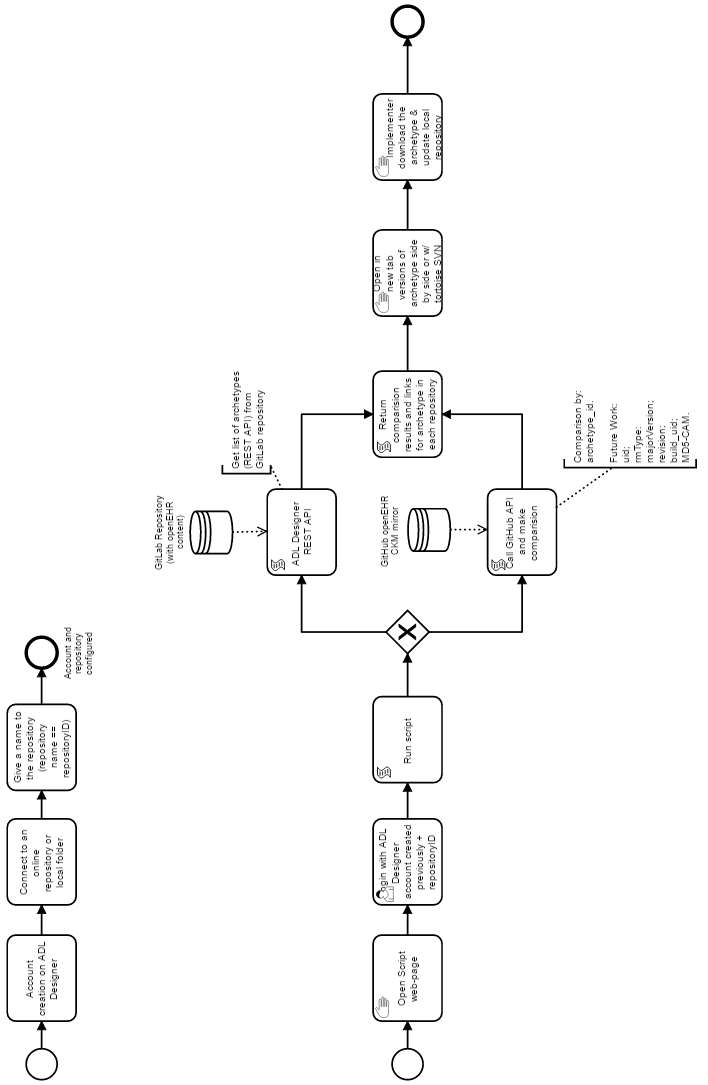
\includegraphics[width=1.07\textwidth]{img/script_process.PNG}
	\caption{Script Process}
	\label{fig:script_process}
\end{figure}

\section{Development}
The script developed was based on the information taken from the objects retrieved by the REST API GET calls of archetypes and templates from ADL Designer to the local repository and from the structure study of openEHR CKM on GitHub, available on Chapter 3 - OpenEHR CKM. The information is analyzed by the script and returns the URL's from the updated archetype versions available at openEHR CKM mirror account. At this stage, the script only analyze and presents the archetypes from the openEHR CKM instance of the openEHR Foundation (Publisher Namespace: org.openEHR) and only present at the "local" folder (see image \ref{fig:CKM_mirror_organization}).

 The classes created to received the information from the calls are presented at table \ref{tab:adl_designer_calls}, together with an example of the data received by each parameter.

\begin{table}[H]
\caption{Classes "Archetypes" and "Templates" used to get information from ADL Designer calls}
\label{tab:adl_designer_calls}
\centering
\begin{tabular}{l}
\toprule[2pt]
\begin{lstlisting}[language=java]
  
  export class Archetypes {
  
    dataResponse: string;  		// full response from ADL Designer
    archetypeId: string; 	 	// e.g. openEHR-EHR-SECTION.adhoc.v1
    path: string; 			// e.g. openEHR-EHR-SECTION.adhoc.v1.adl
    rmType: string; 			// e.g. SECTION
    uid: string; 			// e.g. a82233b9-7f2d-4dd5-8db4-37f6963cfd8c
    details: ["MD5-CAM-1.0.1"]; build_uid; revision: string;
    dependsOn;
    specializedArch : string;
    urlGithubReturn;
    sumArchError;
    sumArchOK : number;
    temp_val;
    
  }


  export class Templates {
  
    dataResponse: string;  		// full response from ADL Designer
    templateId: string;  		// e.g. Vital Signs Measurement Request
    uid: string; 			// e.g. aa69c166-ebbd-48d2-bbfe-9fba97ddfbea
    dependsOn;
    archetypes;
    temp_val;
    
  }
  
\end{lstlisting}
\tabularnewline \bottomrule[2pt]
\end{tabular}
\end{table}

Owing to the repository chosen for testing and proof of concept be connected to a local database hosted at GitLab, the "archetypeID", "path" and "rmType" parameters allowed to construct and retrieve the URL link for each archetype for future comparison. Since it is a private repository, it will require credentials for authentication. 

For the searching component on the openEHR CKM mirror repository, the "rmType" parameter allowed to decide on which URL the archetype should be searched. In case on archetypes with the "rmType" paramater equal to "ACTION", "EVALUATION", "OBSERVATION", "INSTRUCTION" and "ADMIN\_ENTRY", the URL from GitHub should have appended the folder "Entry". In the other "rmType" cases, this was not necessary. The management of both cases can be seen in table \ref{tab:code_calls}. 

\begin{table}[H]
\caption{GET method calls and transformations}
\label{tab:code_calls}
\centering
\begin{tabular}{l}
\toprule[2pt]
\begin{lstlisting}[language=java]
(...)
      this.http.get(githubBaseUrl + this.archetypeLists[i].rmType.toLowerCase() + '/' + 
      this.archetypeLists[i].archetypeId + '.adl', options)
        .subscribe(
        
        response1 => {
          archetypeLists[i].temp_val = response.text().startsWith('archetype') ? imgOk + 
          statusUpd : imgNotOk + statusOut;
        },

        response2 => {
          if (this.archetypeLists[i].rmType.toLowerCase() === 'action' || 'observation' || 
          'admin_entry' || 'evaluation' || 'instruction') {
            this.http.get(githubBaseUrl + 'entry/' + 
            this.archetypeLists[i].rmType.toLowerCase() + '/' + 
            this.archetypeLists[i].archetypeId + '.adl')
              .subscribe(
              response => {
                archetypeLists[i].temp_val = response.text().startsWith('archetype') ? imgOk + 
                statusUpd : imgNotOk + statusOut;
              },
(...)
\end{lstlisting}
\tabularnewline \bottomrule[2pt]
\end{tabular}
\end{table}




\section{Results}

\begin{figure}[H]
	\centering
    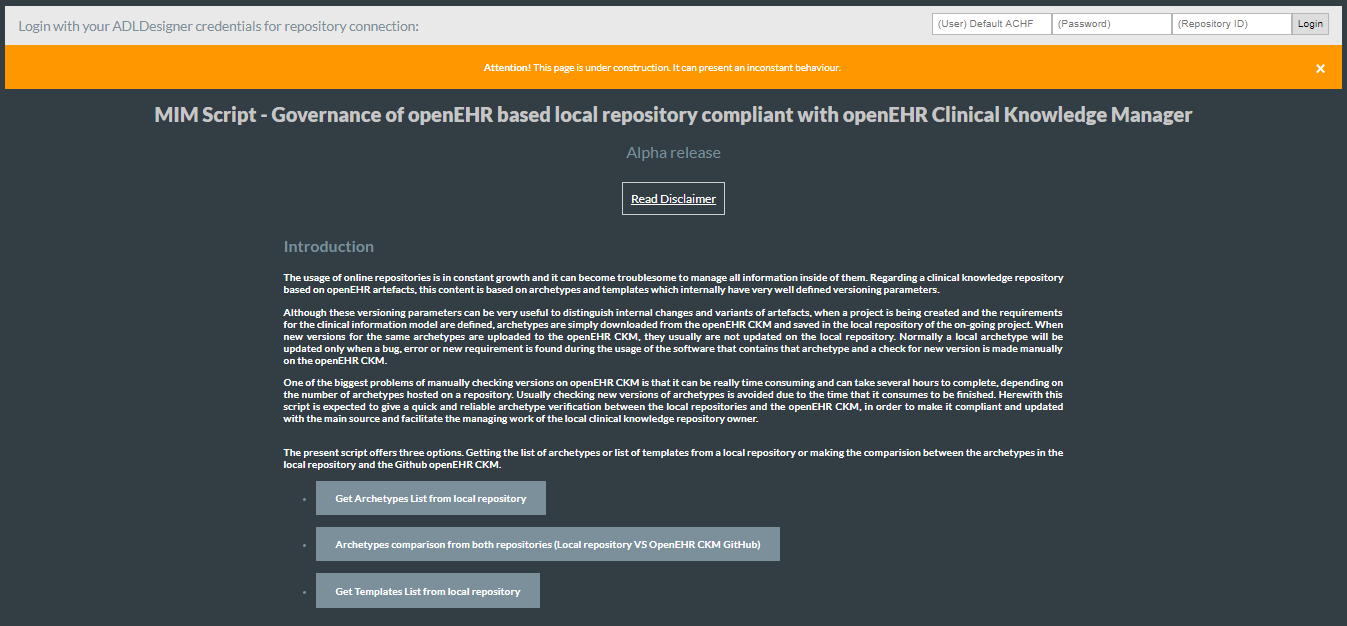
\includegraphics[width=1\textwidth]{img/script_main_page.PNG}
	\caption{Script Main Page }
	\label{fig:script_main_page}
\end{figure}

\begin{figure}[H]
	\centering
    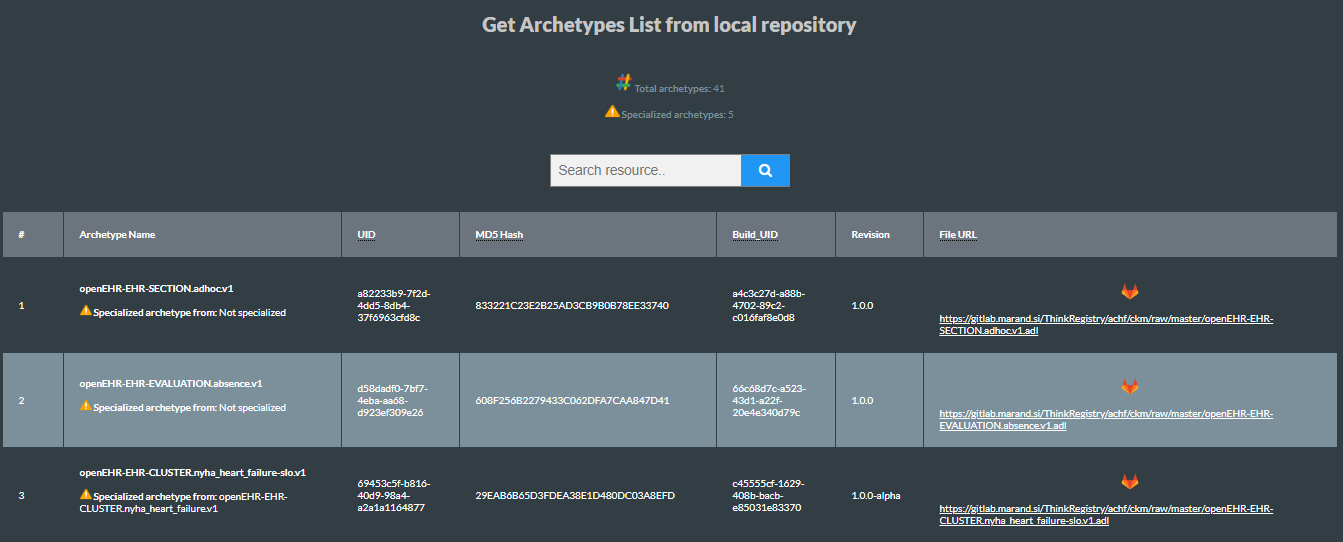
\includegraphics[width=1\textwidth]{img/get_arch_list.PNG}
	\caption{Module Get Archetypes list from local repository }
	\label{fig:get_arch_list}
\end{figure}

\begin{figure}[H]
	\centering
    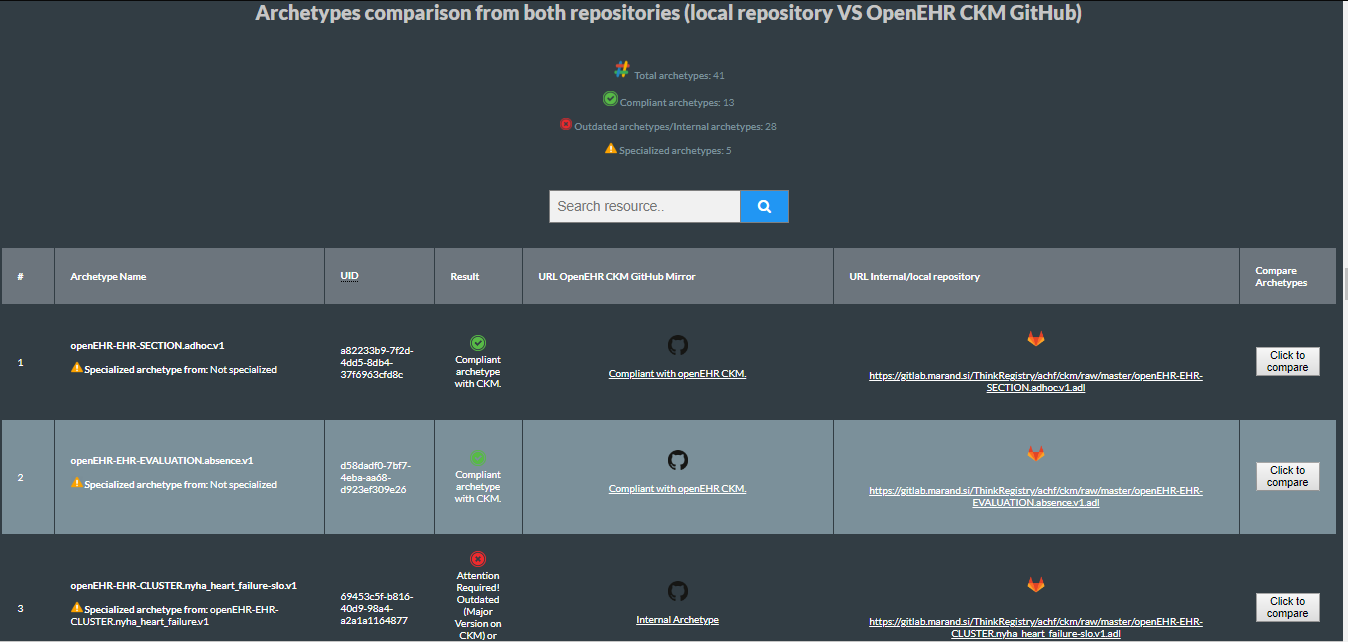
\includegraphics[width=1\textwidth]{img/arch_comparison.PNG}
	\caption{Module Comparison from local repository and compliance with the openEHR CKM mirror at Github}
	\label{fig:arch_comparison}
\end{figure}

\begin{figure}[H]
	\centering
    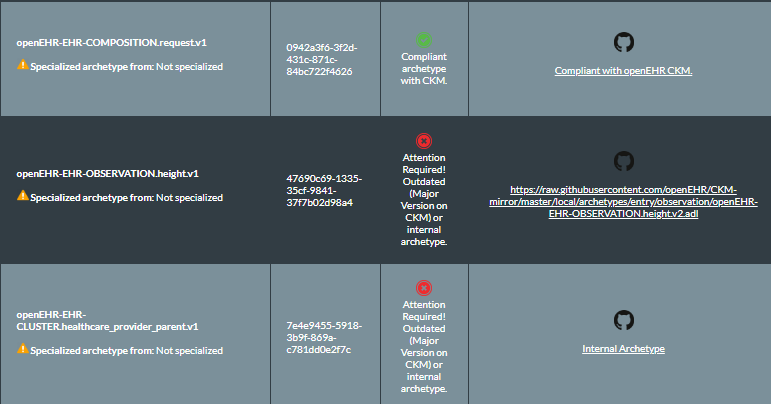
\includegraphics[width=1\textwidth]{img/arch_comparison_2.PNG}
	\caption{Detail from comparison module, with distinction from internal, outdated and compliant archetype}
	\label{fig:arch_comparison_2}
\end{figure}

As a request for improvement, an method for retrieving the list of templates and the set of archetypes included on that templates was also added. 

\begin{figure}[H]
	\centering
    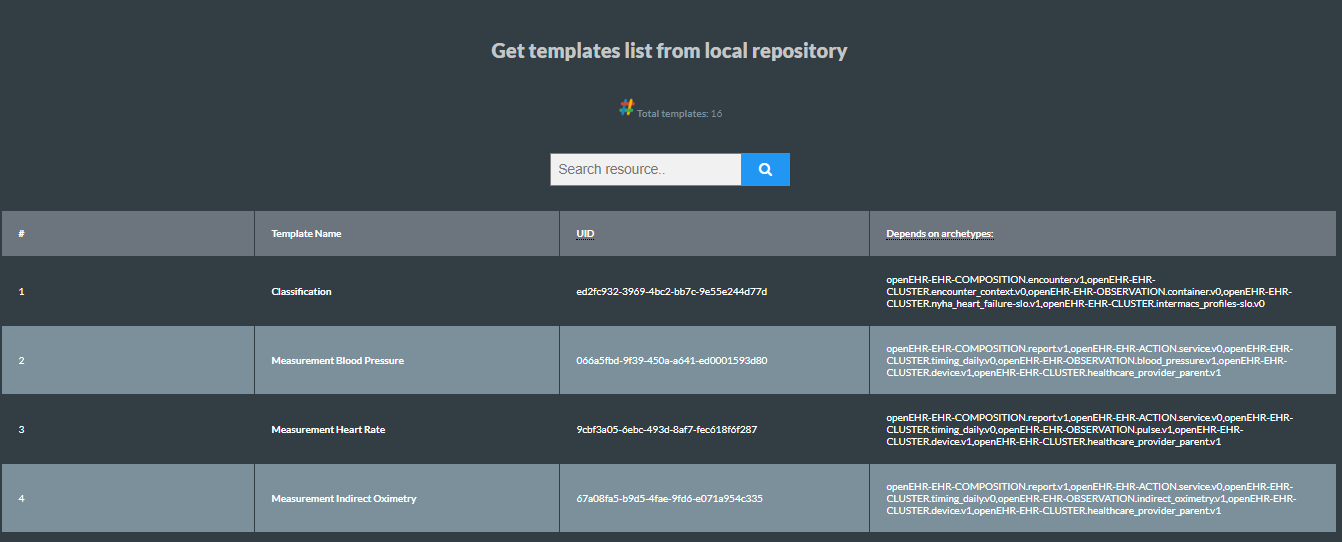
\includegraphics[width=1\textwidth]{img/get_temp_list.PNG}
	\caption{Module Get Templates list from local repository }
	\label{fig:get_temp_list}
\end{figure}

\subsection{Performance}

\end{document}
